\documentclass[a4paper,12pt,oneside]{book}
\usepackage[utf8]{inputenc}
\usepackage[T1]{fontenc}
\usepackage[frenchb]{babel} 
\usepackage{a4wide}
\usepackage{graphicx, float}
\graphicspath{{images/}}
\usepackage{subfig}
\usepackage{tikz}
\usetikzlibrary{shapes,arrows}
\usepackage{pgfplots}
\pgfplotsset{compat=newest}
\pgfplotsset{plot coordinates/math parser=false}
\newlength\figureheight
\newlength\figurewidth
\pgfkeys{/pgf/number format/.cd,
set decimal separator={,\!},
1000 sep={\,},
}
\usepackage{ifthen}
\usepackage{ifpdf}
\ifpdf
\usepackage[pdftex]{hyperref}
\else
\usepackage{hyperref}
\fi
\usepackage{color}
\hypersetup{%
colorlinks=true,
linkcolor=black,
citecolor=black,
urlcolor=black}
\renewcommand{\baselinestretch}{1.05}
\usepackage{fancyhdr}
\pagestyle{fancy}
\fancyfoot{}
\fancyhead[LE,RO]{\bfseries\thepage}
\fancyhead[RE]{\bfseries\nouppercase{\leftmark}}
\fancyhead[LO]{\bfseries\nouppercase{\rightmark}}
\setlength{\headheight}{15pt}

\let\headruleORIG\headrule
\renewcommand{\headrule}{\color{black} \headruleORIG}
\renewcommand{\headrulewidth}{1.0pt}
\usepackage{colortbl}
\arrayrulecolor{black}

\fancypagestyle{plain}{
  \fancyhead{}
  \fancyfoot[C]{\thepage}
  \renewcommand{\headrulewidth}{0pt}
}

\makeatletter
\def\@textbottom{\vskip \z@ \@plus 1pt}
\let\@texttop\relax
\makeatother

\makeatletter
\def\cleardoublepage{\clearpage\if@twoside \ifodd\c@page\else%
  \hbox{}%
  \thispagestyle{empty}%
  \newpage%
  \if@twocolumn\hbox{}\newpage\fi\fi\fi}
\makeatother

\usepackage{amsthm}
\usepackage{amssymb,amsmath,bbm}
\usepackage{array}
\usepackage{bm}
\usepackage{multirow}
\usepackage[footnote]{acronym}


\begin{document}

%%%%%%%%%%%%%%%%%%
%%% First page %%%
%%%%%%%%%%%%%%%%%%

\begin{titlepage}
\begin{center}


\includegraphics[width=0.6\textwidth]{dpt-info-fds.png}\\[1cm]

{\large Licence Informatique 2\up{ème} année - Groupe B}\\[0.5cm]

{\large HLIN405 - TER L2}\\[0.5cm]

% Titre
\rule{\linewidth}{0.5mm} \\[0.4cm]
{ \huge \bfseries Projet PongIO \\[0.4cm] }
\rule{\linewidth}{0.5mm} \\[1.5cm]

% Auteur et Superviseur
\noindent
\begin{minipage}{0.4\textwidth}
  \begin{flushleft} \large
    \emph{Auteurs :}\\
    M. Florian \textsc{Bouffard-V.}\\
    M. Lee \textsc{Gertseen}\\
    M. Alexi \textsc{Husson}\\
    M. Hamza \textsc{Mellouki}\\
  \end{flushleft}
\end{minipage}%
\begin{minipage}{0.4\textwidth}
  \begin{flushright} \large
    \emph{Encadrant :} \\
    M. Jocelyn \textsc{Thiebaut}
  \end{flushright}
\end{minipage}

\vfill

% Bas de page
{\large PongIO - Version 0.8\\ \today}

\end{center}
\end{titlepage}


%%%%%%%%%%%%%%%%%%%%%%%%%%%%%%%%%%%%%%%%%%%%
%%%         Table des matières           %%%
%%%%%%%%%%%%%%%%%%%%%%%%%%%%%%%%%%%%%%%%%%%%
\renewcommand{\contentsname}{Table des matières}
\tableofcontents{}
\addcontentsline{toc}{chapter}{Table des matières}


%%%%%%%%%%%%%%%%%%%%%%%%%%%%%%%%%%%%%%%%%%%%
%%%         Contenu du rapport           %%%
%%%%%%%%%%%%%%%%%%%%%%%%%%%%%%%%%%%%%%%%%%%%

\mainmatter

\pagestyle{fancy}

\cleardoublepage

\chapter*{Introduction}
\addcontentsline{toc}{chapter}{Introduction}
\markboth{Introduction}{Introduction}
\label{chap:introduction}

Cette année, nous avons eu pour tâche de nous rassembler par groupe afin d'effectuer un projet TER tout au long du second semestre. Dans le cadre de ce dernier, nous avons eu l'opportunité d'avoir un enseignant et/ou chercheur nous encadrant. Celui-ci nous aidait alors chaque semaine lors de réunions sur certains points du projet, nous permettant, la plupart du temps, de nous débloquer et de nous aider à nous avancer sur la suite du projet en nous répartissant au mieux les tâches. \newline
Notre travail était donc porté sur un casse-tête appelé "Hashiwokakero" ou plus simplement "Hashi". Ainsi nous avons eu pour but de créer son résolveur afin de le résoudre le plus efficacement possible à l'aide de nos connaissances en algorithmique et en programmation C++. \newline
Concernant le déroulement du projet, nous avons choisi de concentrer notre programme sur GitHub. Ce choix a eu deux différentes raisons de naître, la première concernait l'utilisation de Git qui nous permettait alors de synchroniser le travail effectué à la fin de chaque session de programmation et la deuxième concernait le côté pratique puisque nous pouvons ainsi partager le travail entre nous, étudiants et encadrant, afin que ce dernier puisse voir notre avancement et que nous puissions voir celui de l'autre. \newline
De ce fait, tout cela nous a mené à créer notre projet et son rapport dont voici le plan. \newline
Tout d'abord, nous allons aborder les domaines de l'informatique dans lequel se situe notre projet en les présentant. Puis nous nous attarderons sur le problème précis sur lequel nous avons travaillé. Ensuite, nous assisterons à la description détaillée et expliquée de notre travail. Et pour finir, nous achèverons sur une conclusion faisant part de nos perspectives ouvertes par notre projet ainsi que l'avenir du programme. Nous pouvons aussi trouver à la toute fin de ce rapport, des remerciements ainsi que la bibliographie regroupant les ouvrages sur lesquels nous nous sommes appuyés.
\chapter{Description du projet PongIO}
\label{chap:premier chapitre}

\section{État de l'art}
Le jeu Pong est un des premiers jeux d'arcade mais le tout premier en rapport avec le sport. Le jeu fut développé et commercialisé par Atari en Novembre 1972. Les règles du jeu sont très simples : chaque joueur s'affronte en déplaçant la raquette de haut en bas, via un bouton rotatif, de façon à renvoyer la balle dans le but adverse. Le joueur peut changer la direction de la balle en fonction de l'endroit où celle-ci tape sur la raquette, alors que sa vitesse augmente graduellement au cours de la manche. Un score est affiché pour la partie en cours et des bruitages accompagnent la frappe de la balle sur les raquettes. C'est donc un jeu inspiré du tennis de table en vue du dessus dont voici une illustration:

\begin{figure}[H]
  \center
  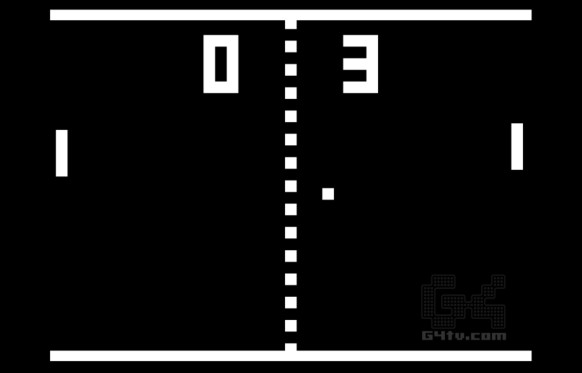
\includegraphics[width=5cm]{images/pong}
  \centering
  \caption{Illustration du jeu Pong. On voit à droite les rectangles correspondant aux raquettes des joueurs. La balle correspond au carré blanc proche du centre de l'image. Le score est affiché en haut de l'écran.}
  \label{fig:une-image}
\end{figure}


Le jeu à d'ailleurs rapporté plus de 40 millions de dollars de chiffres d'affaires en 1975. Ce succès est considéré comme l'évènement précurseur de l'industrie du jeu vidéo. Notre choix s'est porté sur ce jeu pour cette même raison. C'est également dans le but de tester nos compétences en programmation que nous nous sommes fixés comme but de donner à ce jeu "classique" une touche moderne et innovatrice, c'est pourquoi nous avons décidé d'en faire un jeu ".io".\\
Les jeux ".io" ont vu le jour grâce au jeu d'action massivement multijoueur AgarIO dont le succès fut tout simplement fulgurant. En effet durant sa première année de sortie il fut l'un des jeux les plus populaires que soit pour son site ou pour son application mobile. Dans ce jeu le joueur contrôle une cellule dans une carte où il doit manger un maximum de cellules pour devenir le plus gros possible. Puis de nombreux autres jeux ont suivi la tendance comme SlitherIO, VertixIO et plusieurs autres. Il y a de nombreuses raisons au succès de ses différents jeux ".io". Tout d'abord l'accessibilité de ces jeux les rend jouables n'importe où dans le monde. Le domaine ".io" dorénavant culte est très simple a mémoriser pour la majorité des gens. De plus, son prix n'est pas très élevé pour les développeurs comparé à d'autres domaines, ce qui rend les publicités suffisamment rentable. En effet, la gratuité implique que plus de joueurs peuvent y jouer. Finalement, le plus important, le fait que le jeu soit multijoueur permet aux joueurs du monde entier de s'affronter.\\


\section{Principe du PongIO}


La principale motivation qui nous a poussé à créer PongIO est le désir de moderniser et de redéfinir le mythique jeu qu'est Pong. Ainsi, en conservant les mécaniques de base, nous avons élargi les possibilités de varier les modes de jeu. PongIO ne se limite pas seulement à un affrontement de deux joueurs, nous avons implémenté différents modes de jeu allant du 2 contre 2 à chacun pour soi mais en allant jusqu'à 10 joueurs : ils sont ainsi placé sur un plateau hexagonal.


Nous avons décidé d'accorder une grande importance au graphisme de notre jeu pour qu'il puisse se distinguer suffisamment du Pong classique et qu'il apporte au joueur une expérience de jeu nouvelle et inédite. Nous avons choisi de nous orienter vers un design du jeu pixelisé. Le résultat s'accordait de façon impressionnante à notre idée du design pour la page de lancement du jeu. Voici une illustration de notre écran de lancement de partie:

\begin{figure}[H]
  \centering
  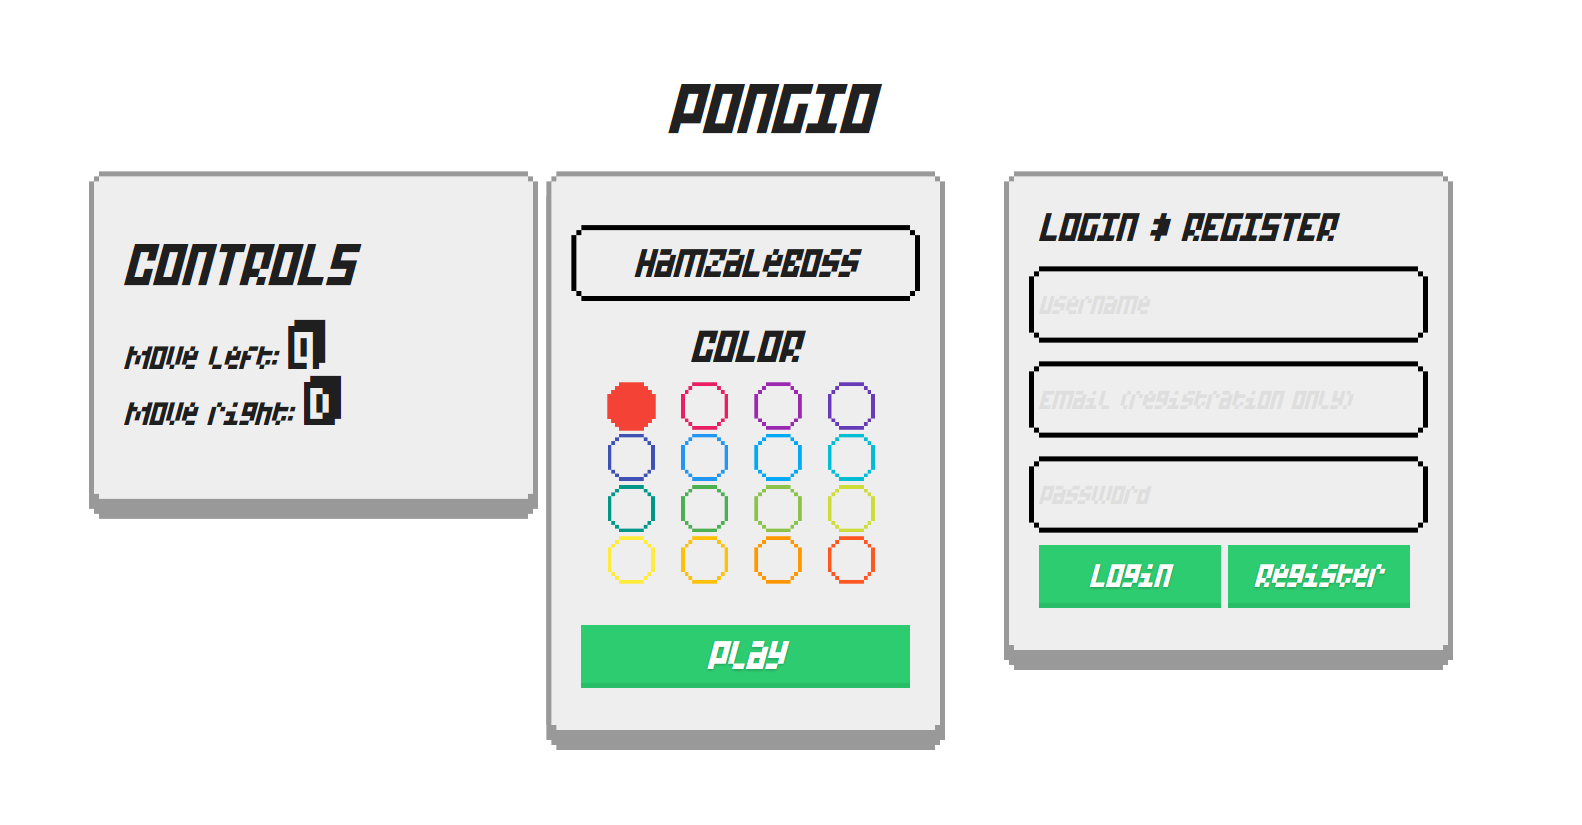
\includegraphics[width=10cm]{images/Capture3}
  \caption{Illustration de notre page de lancement aux graphismes pixélisées. Au centre, on voit le menu qui demande le pseudo et la couleur du joueur. À gauche, on indique les contrôles du jeu. À droite, un formulaire d'inscription et de connexion.}
  \label{fig:deux-image}
\end{figure}

Un de nos objectifs de départ était de permettre une interaction simple et immersive entre les joueurs durant le jeu. C'est donc dans cette optique qu'on a commencé par y intégrer un chat et un classement. On ne souhaitait pas suivre le schéma des autres jeux ".io" mais ces deux aspects nous semblaient essentiels pour l'enrichissement de l'expérience de jeu et des interactions entre joueurs.


Dans la continuité de notre démarche de changement, nous avons complètement changé le style de la fenêtre de conversation et du classement pour les accorder a notre charte graphique. Ce n'était guère notre choix de départ, nous comptions nous orientés vers un design moderne avec fond ébène mais le résultat ne s'accordé pas avec le plateau de jeu en plein milieu. Voici donc une illustration de notre classement et de notre chat pixélisés:

\begin{figure}[H]
  \centering
  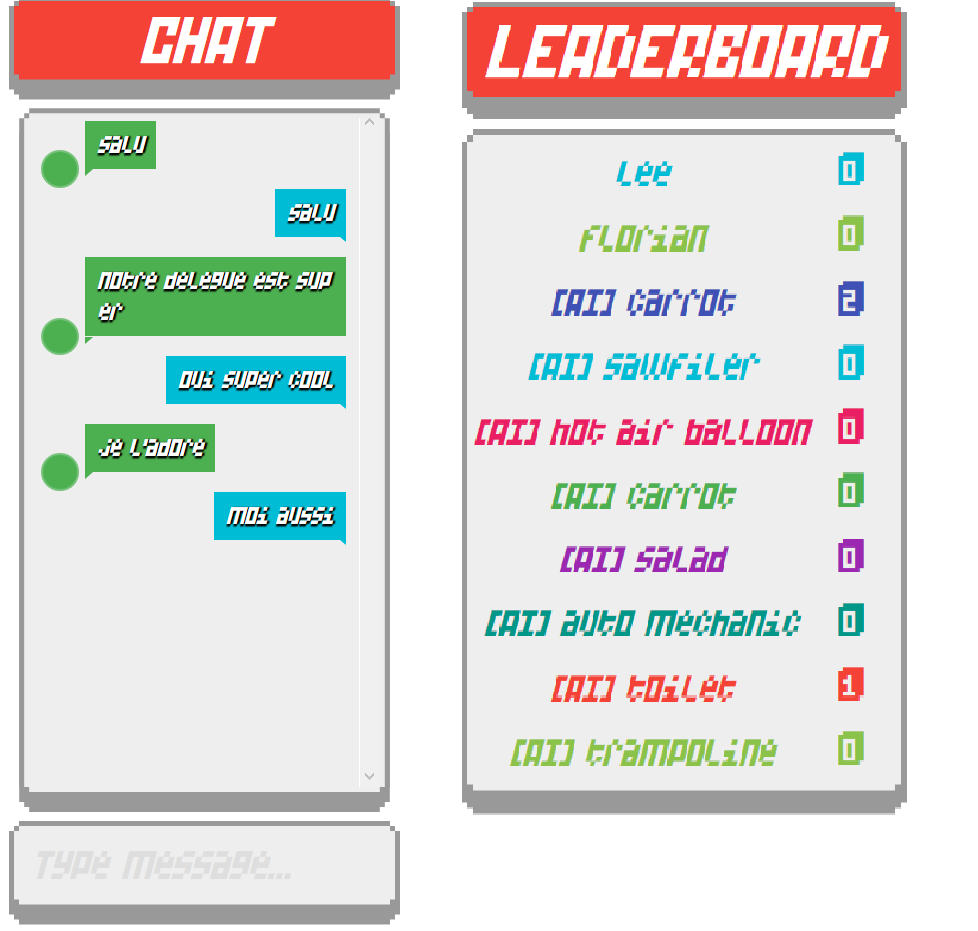
\includegraphics[width=10cm,height=7cm]{images/Capture6}
  \caption{Illustration de notre chatbox à gauche et de notre classement à droite.}
  \label{fig:trois-image}
\end{figure}

Finalement nous avons implémenté de multiples modes de jeu qui alternent après une partie de deux minutes. Pour permettre ce changement nous avons ajouté un compte à rebours juste en dessous de notre classement. Les modes de jeu se composent alors d'un mode 1vs1 simple, en d'autres termes, le mode dit "classique", un mode 2vs2 pour qui voient s'affronter deux équipes de deux joueurs, un mode avec 5 joueurs en forme d'hexagone et un mode avec 10 joueurs en forme de décagone. Voici une représentation des différents modes implémentés dans notre jeu:

\begin{figure}[!h]
  \centering
  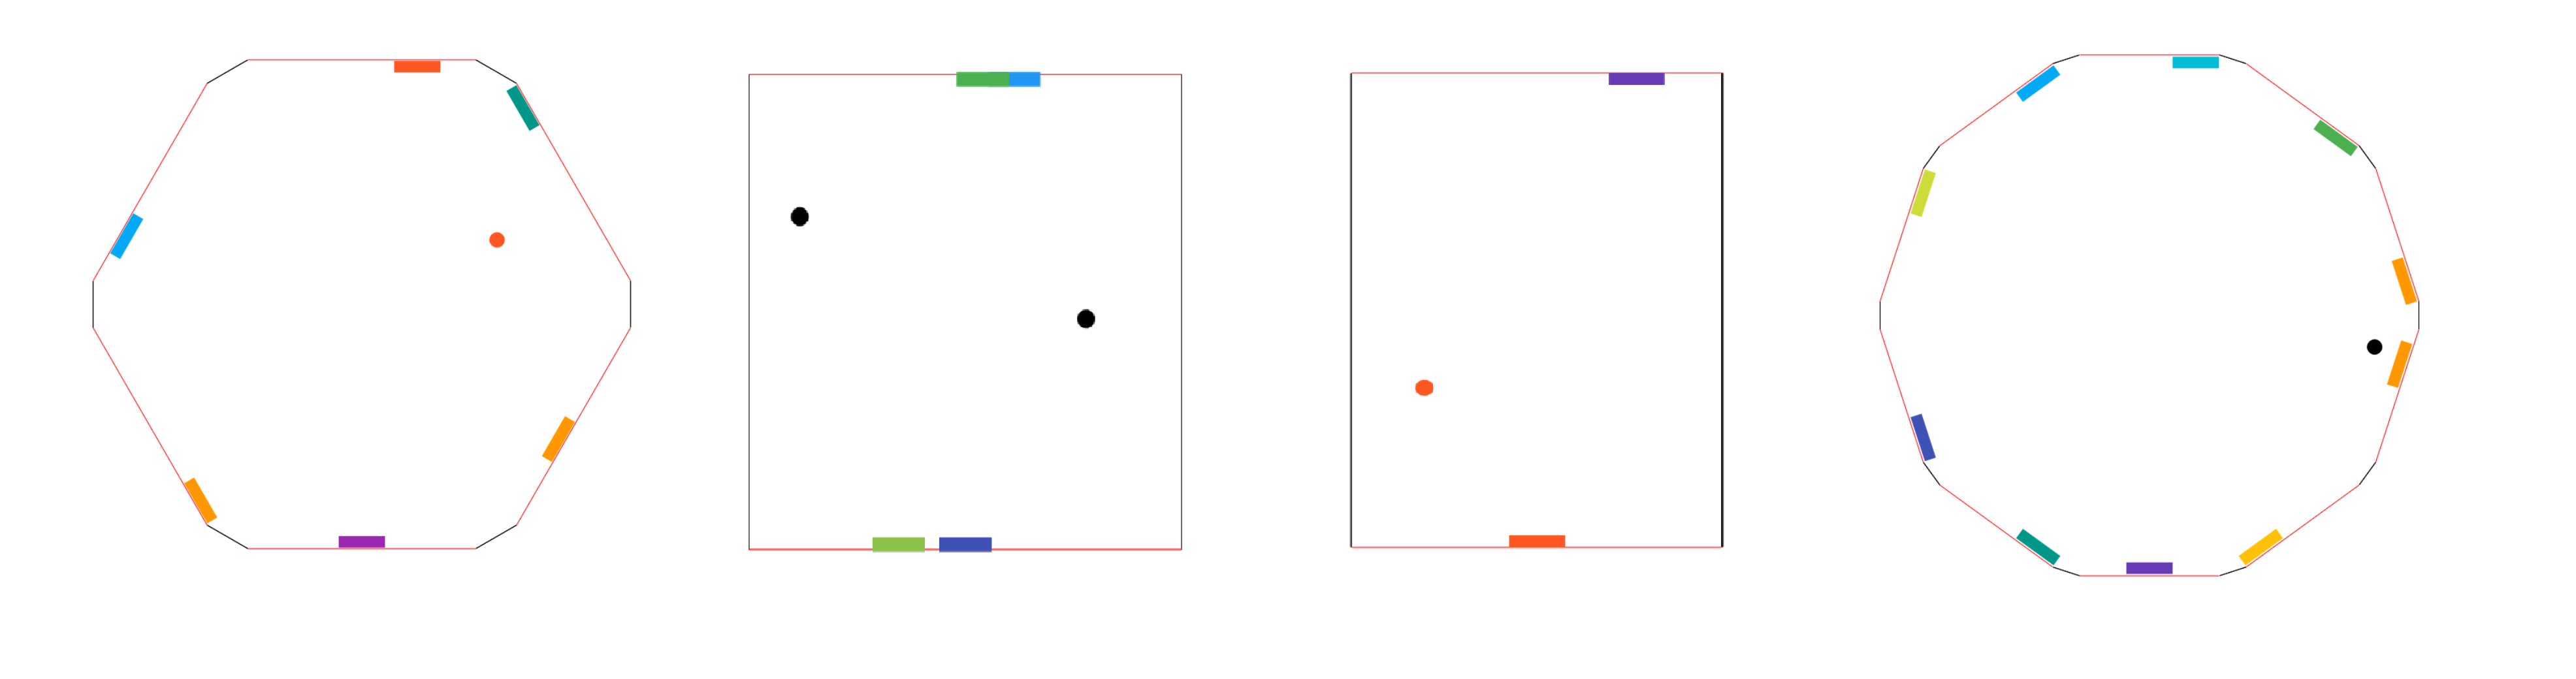
\includegraphics[width=15cm]{images/Capture11}
  \caption{Illustration des différents modes.}
  \label{fig:quatre-image}
\end{figure}


\section{Gestion du projet}

À la différence de plusieurs autres groupes de TER qui ont utilisé la méthode classique de gestion de projet, nous avons développé notre projet grâce à la méthode agile.


La méthode agile utilise le concept de développement itératif qui consiste à découper le projet en plusieurs parties que l’on appelle \emph{itérations} ou \emph{sprints}.


Ces \emph{sprints} sont en fait des sous-projets prédéfinis à l'avance avec les membres du groupe ou éventuellement avec le client en précisant les différentes parties qui seront développées en priorité. Avec le professeur référant, le groupe établit alors les tâches nécessaires pour le développement de ces parties.


Le but est de découper le projet en "itérations" plutôt que de tout prévoir et planifier tout en sachant que des imprévus arriveront en cours de route.\\
Les avantages du développement itératif sont avant tout une meilleure qualité de la communication entre les membres du groupe ou possiblement le client avec la possibilité de clarifier les exigences de chacun au fur et à mesure, une meilleure visibilité pour le groupe ou le client sur l’avancement des différentes tâches, un meilleur contrôle de la qualité car les tests du code sont effectués en continu, une meilleure détection des risques car les risques seront détectés plus tôt; une motivation et une confiance entre le groupe dû entre autres à la satisfaction d’avoir atteint un objectif fixé et enfin un contrôle des coûts plus minutieux car ainsi le projet peut être arrêté s’il n’y a plus de budget.


Notre projet a tout de suite démarré par la création d'un compte GitHub pour mieux gérer le partage du travail dans tout le groupe et pour permettre une meilleure coordination entre chacun de nous. GitHub est un site d'hébergement et de gestion de code source. De plus nous avons chacun travaillés sur des branches différentes pour éviter de saturer et de fausser notre code principal.
\chapter{Élaboration du Projet}
\label{sec:unchapitre}

Dans ce chapitre nous allons détailler comment c'est réellement déroulé l'élaboration de notre projet au cours du temps.

\section{L'implémentation du jeu}

\subsection{Les technologies utilisées}

Nous avons choisi de travailler avec Javascript comme langage de programmation afin de mieux appréhender l'aspect multijoueur en temps réel de notre jeu. Javascript est un langage de programmation de scripts principalement utilisé pour les sites interactifs et les serveurs avec l'utilisation de Node.js. En outre ce n'est pas un langage compilé mais un langage interprété. D'ailleurs puisqu'aucun d'entre nous n'avait programmé en Javascript, nous avons dû acquérir les bases de celui-ci de manière autodidacte. Nous avons également dû travailler avec les langages que sont HTML et CSS pour modeler l'affichage et l'aspect graphique de notre jeu.

Nous avons changé l'esthétique du jeu, en modifiant l'affichage et l'interface graphique, et augmentant le nombre de joueurs simultanées en créant différents plateaux de jeu en forme de polygone et en y ajoutant différentes interactions multijoueur. La partie la plus difficile à ce niveau du projet était de créer un jeu en temps réel pour cela nous nous sommes tourné vers SocketIO. Il s'agit d'une librairie de Javascript qui permet de créer des applications web en temps réel. En d'autres termes, elle permet la communication en temps réel entre le client et le serveur. Avec une partie client exécutée par le navigateur et une partie serveur gérée par Node.js. Cette librairie présente trois avantages majeurs, tout d'abord sa simplicité puis sa prise en charge et sa probabilité sur la majorité des navigateurs incluant même les vieux navigateurs.


Pour l'hébergement du jeu sur un serveur nous nous sommes tournés vers Heroku qui est considéré comme l'un des plus anciens services de cloud-computing. Le cloud-computing est l'exploitation de la puissance de calcul ou de stockage de serveurs informatiques distants par l'intermédiaire d'un réseau. Nous avons donc choisi Heroku car il permet le déploiement très rapide d'applications web dans le cloud mais aussi pour sa gratuité tant que l'application n'est pas monétisé.


\subsection{Organisation interne du jeu}

Nous avons développé toutes les classes nécessaires au bon déroulement du jeu. Ces classes sont donc la classe \emph{player} qui gère le joueur, la classe \emph{ball} qui comme son nom l'indique régit la balle et ses actions, la classe \emph{map} qui crée tous les murs et buts de façon spécifique selon le plateau, les classes \emph{wall} et \emph{goal} qui gère le calcul de la bonne rotation des murs et des buts dans le jeu, la classe \emph{helpers} contenant toutes les fonctions nécessaire au projet, la classe \emph{express} qui crée le lien entre le client et le serveur,  la classe \emph{game} qui implemente la partie en manipulant les classes précédemment citées, la classe\emph{gameserver} qui gère la création de toutes les parties du jeu et enfin la classe \emph{SocketIO} qui gère l'envoie des données entre le client et le serveur.\\

\section{Un point du projet plus en détail : L'intelligence artificielle}

Afin qu'un joueur seul puisse jouer dans l'attente de trouver un adversaire humain, nous avons commencé à implémenter une intelligence artificielle (IA) pour le jeu. Cette phase fut très difficile car il fallait être suffisamment pointilleux pour que l'IA soit fonctionnelle avec tous les modes de jeu que nous comptions mettre en place. Il fallait aussi qu'elle puisse réagir différemment selon la situation. C'est-à-dire que l'IA doit être capable de viser un espace vide des buts adverses plutôt que de renvoyer bêtement la balle. D'ailleurs un aspect très intéressant de l'intelligence artificielle c'est son évolution au cours de notre projet. Et comment chaque changement sur son algorithme la façonnait lui permettant d'être meilleure et imprévisible. Nous avons même créé un mode sans vue pour pouvoir comparer son évolution au cours de notre projet en les faisant s'affronter les unes contre les autres sur des parties plus ou moins longues.


Au cours de la réalisation et de l'implémentation de l'IA, nous avons rencontré divers problèmes, le premier lié au remplacement d'une IA par un joueur puis un second lorsque l'IA devait reprendre sa place.


L'aire de jeu est représentée par un polygone qui varie en fonction du nombre de joueurs et du mode de jeu. De ce fait, un joueur qui se connecte dans une nouvelle partie se voit en bas de l'écran, ses contrôles gauche et droite sont dans le même sens que sa raquette. Les autres participants sont remplacés par des IA. Cependant, si un autre joueur se connecte à cette même partie, celui-ci prendra la place d'une IA, c'est-à-dire sur le côté ou même en haut du plateau. Néanmoins, ce nouveau joueur aurait la même vue du jeu que le premier, désaxée par rapport à sa raquette, rendant l'utilisation du clavier trop difficile. Pour pallier à ce problème, nous avons ajouté à notre code un algorithme qui pour chaque joueur, effectue une rotation de l'affichage afin que chaque joueur se voit en bas du plateau.


Un autre problème que nous avons rencontré est lié aux joueurs qui quittent une partie en cours. En effet ces joueurs n'étaient pas toujours remplacés par un nouveau joueur en attente de jouer et le changement de plateau n'était guère envisageable car trop brutale et peu immersive pour les autres joueurs. Nous avons fait en sorte que ce joueur soit alors toujours remplacé par une intelligence artificielle qui prendrait alors le relais sans changer son score.

\subsection{Les différentes versions de l'IA}

Nous avons tout d'abord implémenté une première version de notre IA. Le but de cette IA n'était pas d'intercepter la balle mais de se déplacer de façon aléatoire. Les objectifs de cette démarche étaient multiple. D'une part, elle nous a permis d'appréhender les contraintes en terme de programmation d'avoir une IA (quelles sont les classes nécessaires, quand est-ce qu'on doit faire le calcul du mouvement, etc...). D'autre part, cette IA permettait de nous donner une première version, à laquelle nous feront affronter les prochaines versions plus complexes. Cette IA est donc dite "naïve" car son mouvement ne dépend pas de la balle.


C'est ensuite dans l'optique de créer une IA meilleure que nous avons développé l'algorithme d'une nouvelle IA: l'IA défensive. Le but était de permettre à l'IA de calculer le lieu de la prochaine interception entre ses propres buts et les différentes balles selon le cas de figure. Cette IA fut un réel succès dû à son algorithme de prédiction qui était capable de déterminer le lieu de la prochaine interception entre la balle et un but plusieurs secondes a l'avance. Cette IA est donc une IA à caractère purement défensive.


Nous nous sommes finalement lancés dans l'implémentation de l'IA la plus intelligente possible capable donc de viser l'espace vide entre un joueur et le côté de ces buts. Cette tâche fut particulièrement difficile en raison d'un grand nombre de calculs trigonométriques nécessaires à sa bonne réalisation. Cette IA ne se contente donc plus de se placer sur le lieu de l'interception mais elle place le joueur de façon à dévier la balle d'un certain angle pour pouvoir atteindre sa cible. Le caractère cette IA est quant à lui orienter vers l'offensive.\\

% Ajouter un schéma d'un match à 6 joueurs et montrer les différentes trajectoires de balle possible pr l joueur du bas

\clearpage

\subsection{Les résultats comparatifs}

Comme nous l'avons précisé dans la partie précédente, nous avons créé un mode sans vue dans le but d'avoir un meilleur aperçu de l'évolution de notre IA durant le projet. Afin que l'IA défensive ne sois pas trop parfaite et arrête tous les tirs provenant de n'importe quelle IA, nous avons mis en place un pourcentage d'erreur afin qu'elles puissent se prendre des buts.\\

Si dessous un tableau montrant le score entre deux IA pendant le temps indiqué. Les résultats ont été enregistrés à 5, 10 et 20 minutes de jeu.

\begin{table}[ht]
  \begin{center}
    \begin{tabular}{|c|c|c|c|c|}
      \hline
      Affrontements IA / Temps de Jeu (Min) & 5 & 10 & 20\\
      \hline
      IA 1 vs IA 2& 0 / 12 & 1 / 25 & 2 / 48 \\
      \hline
      IA 1 vs IA 3& 3 / 21 & 9 / 49 & 21 / 116 \\
      \hline
      IA 2 vs IA 3& 9 / 4 & 17 / 7 & 22 / 15 \\
      \hline
    \end{tabular}
    \caption{Tableau sur le Mode Sans Vue.}
    \label{tab:un-tableau}
  \end{center}
    IA1 = IA naîve alias \emph{Florian}\\
    IA2 = IA défensive alias \emph{Gertseen}\\
    IA3 = IA offensive alias \emph{Hamza}
\end{table}



%A retoucher avec un exemple ou à enlever

%\section{La physique du rebond}

%Nous avons ensuite dû coder un nouvel algorithme du rebond adapté au mode de jeu en forme de polygone. Ce ne fut pas une tâche aisée car nous avons fait face a de nombreux problèmes de mathématiques. En effet notre travail repose en grande partie sur un canvas implémenté en HTML donc tous les calculs comme le calcul du rebond de la balle nécessite plusieurs formules de trigonométrie. Pour pallier ce problème de mathématique, nous nous sommes rendus dans une salle de la bibliothèque universitaire pour faire un bref rappel sur certaines de ces formules avec l'aide de notre encadrant.\\

\chapter*{Conclusion et perspectives}
\addcontentsline{toc}{chapter}{Conclusion}
\markboth{Conclusion}{Conclusion}
\label{sec:conclusion}


Une amélioration future plus qu'intéressante et déjà entamée par le groupe serait de changer la modélisation de notre jeu via Unity pour pouvoir y jouer avec une vue en 3D. Cette idée serait révolutionnaire pour changer le fait que le Pong ne peut se jouer que sur un plateau en 2D. Voici une brève représentation de ce que donnerait une modélisation de notre jeu sur Unity:

\begin{figure}[ht]
  \centering
  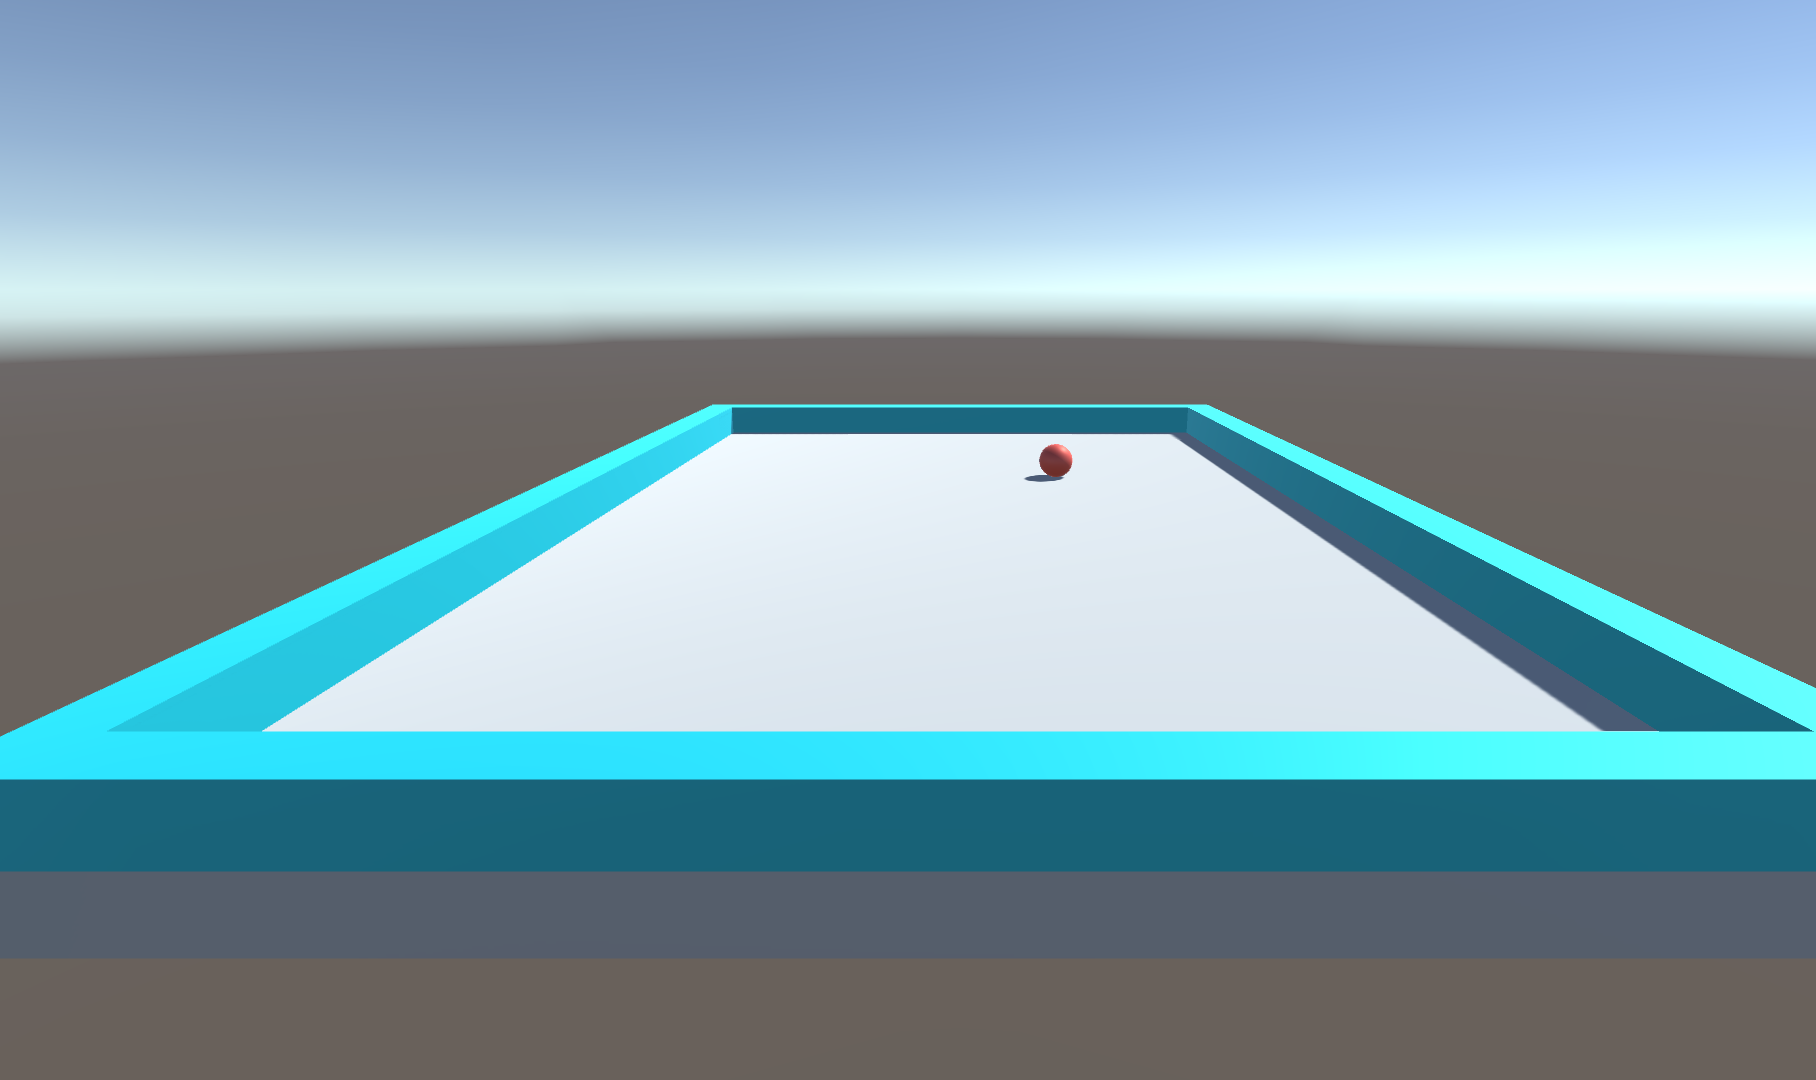
\includegraphics[width=5cm]{images/Capture12}
  \caption{Illustration de notre jeu sur Unity.}
  \label{fig:une-image}
\end{figure}

Cette amélioration nous inspire beaucoup pour l'avenir de notre jeu.\\
Pour conclure, Nous pouvons dire que ce projet fut très enrichissant pour chacun d'entre nous. D'ailleurs nous allons continuer a travailler dessus pour peut-être un jour le rendre public et collecter l'avis des joueurs sur notre vision d'un Pong moderne.


\bibliographystyle{authoryear-fr}
\bibliography{references}

%%%%%%%%%%%%%%%%%%%%%%%%%%%%%%%%%%%%%%%%%%%%
%%%             Bibliographie            %%%
%%%%%%%%%%%%%%%%%%%%%%%%%%%%%%%%%%%%%%%%%%%%
\begin{thebibliography}

\hfill \break


[1] Wikipédia : \\
Pong - https://fr.wikipedia.org/wiki/Pong\\
Heroku - https://fr.wikipedia.org/wiki/Heroku\\
Javascript - https://fr.wikipedia.org/wiki/Javascript
\hfill \break


[2] acces dev : \\
La différence entre méthode agile et méthode classique - http://www.access-dev.com/access-dev/la-gestion-de-projet-methodes-classiques-vs-methodes-agiles
\hfill \break


[3] Tutorialspoint :  \\
Tutorial Javascript - https://www.tutorialspoint.com//Javascript/index.htm\\
Materialize tutorial - http://www.tutorialspoint.com/materialize/
\hfill \break


[4] codeincomplete : \\
Javascript Pong - http://codeincomplete.com/posts/Javascript-pong
\hfill \break


[5] bychat : \\
CSS chat - https://www.bypeople.com/CSS-chat/
\hfill \break

\end{thebibliography}
\clearpage
%%%%%%%%%%%%%%%%
%%% Abstrait %%%
%%%%%%%%%%%%%%%%

\thispagestyle{empty}

\vspace*{\fill}
\noindent\rule[2pt]{\textwidth}{0.5pt}\\
{\textbf{Remerciements ---}}
Nous tenons a remercier toutes personnes ayant aider au projet que ce soit de près ou de loin. Nous remercions également certains membres du groupe B de la licence 2 informatique qui nous ont aidé.
Nous tenons aussi a remercier particulièrement notre encadrant pour toute l'aide qu'il nous a apporté durant la durée du projet.
\\
\noindent\rule[2pt]{\textwidth}{0.5pt}
\begin{center}
    Faculté des Sciences
    Université de Montpellier\\
    Place Eugène Bataillon\\
    34090 Montpellier\\
\end{center}
\vspace*{\fill}

\end{document}